\clearpage

\section{Studies of Jets from Pileup}
\label{sec:pujets}

You can type text and make a paragraph like this. You can reference figures like by doing Fig.~\ref{fig:example}.


% Make comments with the '%' sign
% This is how you make a plot:

\begin{figure}[!h]
\begin{center}
\begin{tabular}{cc}
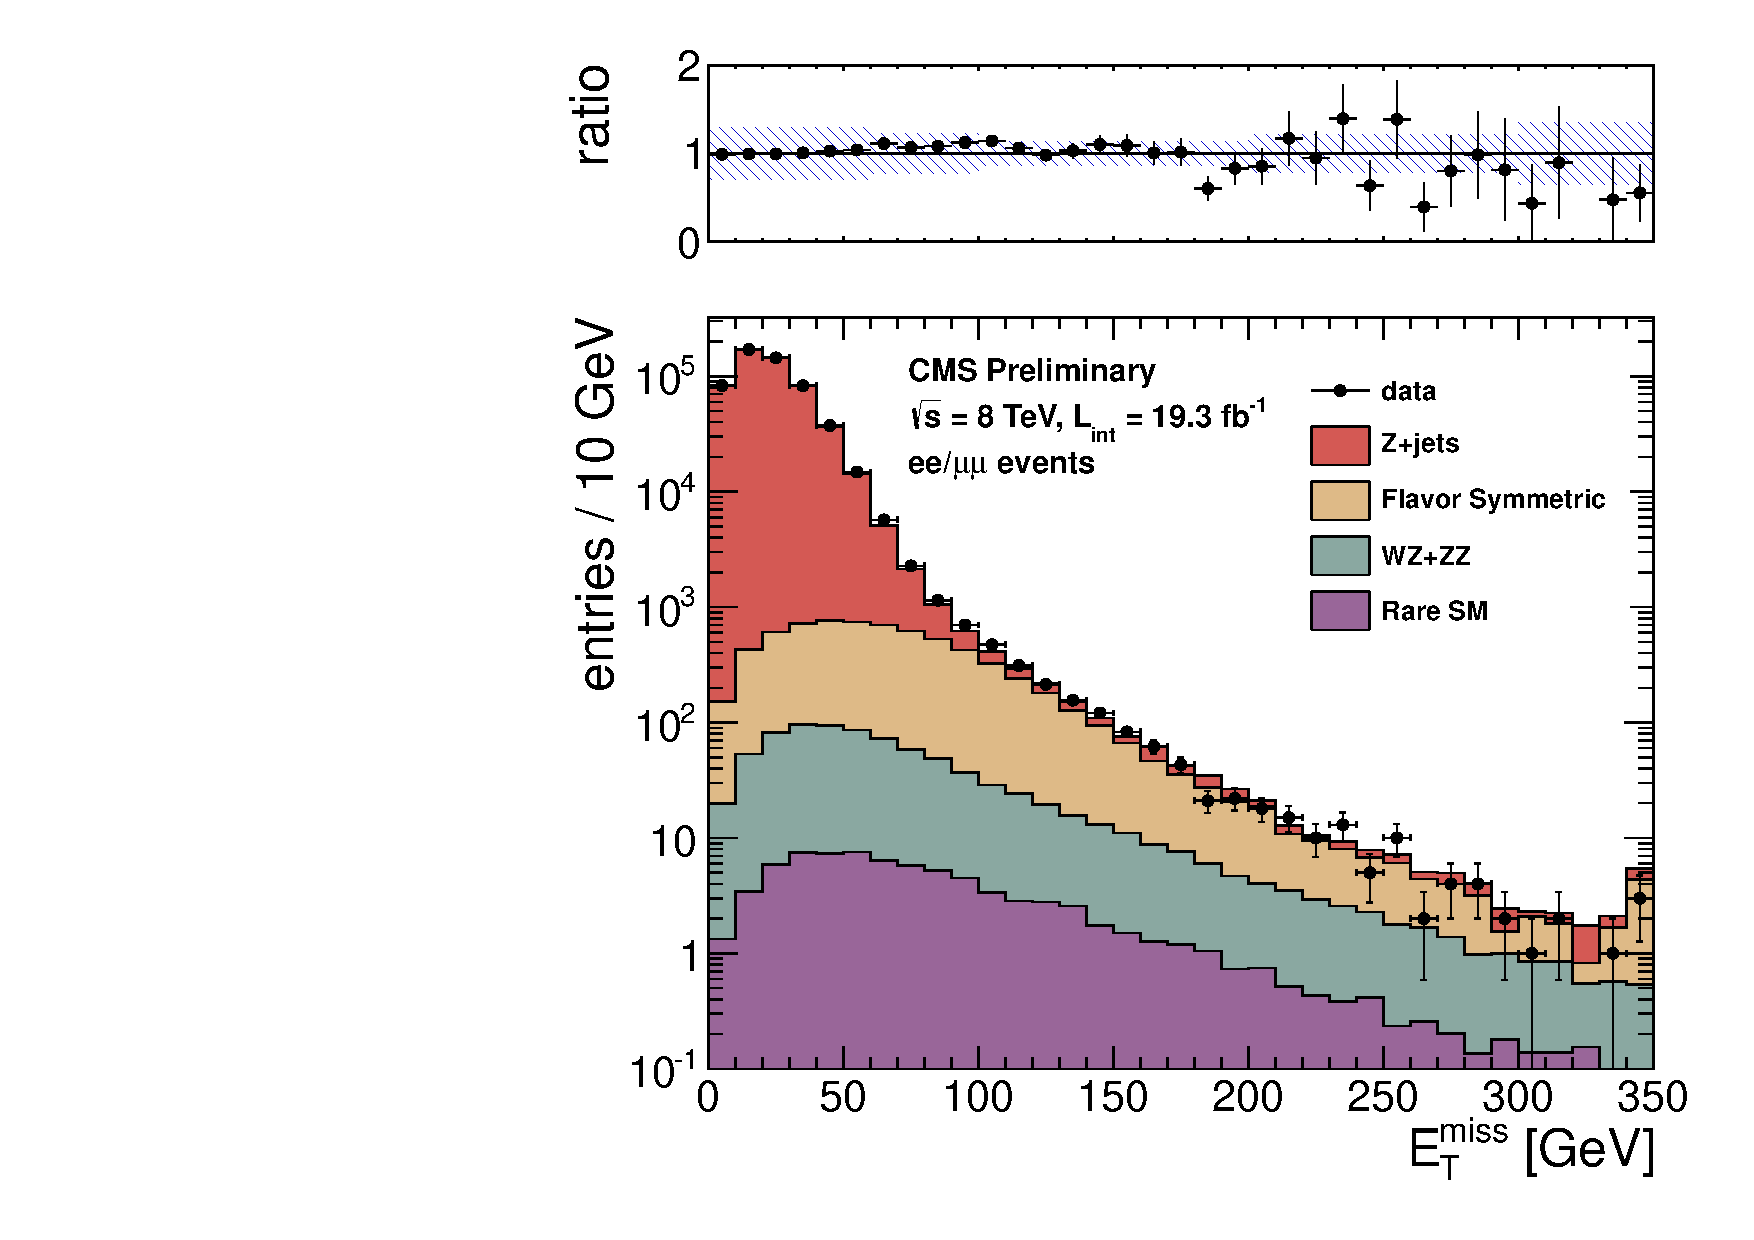
\includegraphics[width=0.6\textwidth]{plots/pfmet_all_19fb.pdf}
\end{tabular}
\caption{This is an example plot and here is where you put the caption.
\label{fig:example}
}
\end{center}
\end{figure}

% This is how you make a table:

\begin{table}[htb]
\begin{center}
\caption{\label{table:example} This is an example table and here is where you put the caption. }
\begin{tabular}{l|cc}
\hline
\hline
Blah & A & B \\
\hline
Row1 & C & D \\
Row1 & E & F \\
\hline
\hline
\end{tabular}
\end{center}
\end{table}

% This is how you make a bulleted list:

\begin{itemize}
\item Item1
\item Item2
\item Item3
\end{itemize}

\clearpage
